% -*- TeX-engine: luatex -*-
\documentclass[dvipsnames,presentation,aspectratio=169,14pt]{beamer}
\usepackage{hastingstheme}
\titlegraphic{
\includegraphics[scale=.35]{static_figures/du_bn.pdf}}
\author{\large Massimiliano Fasi}
\date{}


% \usepackage{template}
% \renewcommand{\authorname}{Lawrence Mitchell\inst{*}}
\renewcommand{\authoremail}{\inst{*}\texttt{lawrence.mitchell@durham.ac.uk}}

% \renewcommand{\sessionnumber}{4}
% \renewcommand{\sessiontitle}{Performance measurements}
% \usepackage{tikz}

\usepackage{pgfplots}
\pgfplotsset{compat=1.15}
\usetikzlibrary{matrix,fit,positioning,calc}
\usepackage{pgfplotstable}
\usetikzlibrary{pgfplots.groupplots}
\date{}

\begin{document}

\title{\firasemibold\color{White}%
  {\fontsize{20}{0}\selectfont SESSION 4\\
    \fontsize{34}{34}\selectfont Performance\\measurements\par}}
\titleslide

% \begin{frame}
%   \frametitle{Roofline of dense matrix--vector product}
%   \begin{center}
%     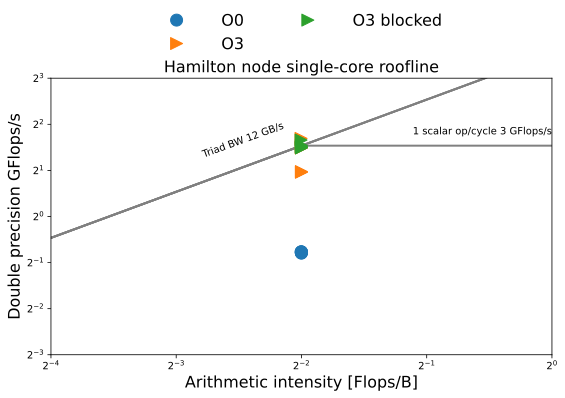
\includegraphics[width=0.9\textwidth]{figures/roofline-dmvm}
%   \end{center}
% \end{frame}

\begin{frame}
  \frametitle{Overview}
  \structure{Roofline}
  \begin{itemize}[itemsep=5pt]
  \item comparison between hardware configurations
  \item high-level overview of code performance
  \item general guidance for optimisation
  \end{itemize}
  \pause
  \vskip 11pt

  \structure{Measurements}
  \begin{itemize}[itemsep=5pt]
  \item to get more information about bottleneck
  \item to confirm the hypothesis formed through roofline analysis
  \end{itemize}
\end{frame}

\begin{frame}
  \frametitle{Performance measurements}
  Special purpose \structure{registers}:
  \begin{itemize}[itemsep=5pt]
  \item common in modern hardware
  \item record low-level performance events
    \begin{itemize}[itemsep=3pt]
    \item number of Flops of different type (scalar, sse, avx)
    \item cache miss/hit counts at various levels
    \item branch prediction success rate
    \item \ldots
    \end{itemize}
  \item<2> can be overwhelming
  \item<2> best used to confirm hypothesis from some model
  \end{itemize}
\end{frame}

\begin{frame}
  \frametitle{Caveats}

  \begin{itemize}[itemsep=8pt]
  \item Information about
    \begin{itemize}[itemsep=3pt]
    \item the algorithm you implemented
    \item the way you implemented it
    \item the data moved in the measured run
    \end{itemize}
  \item Does not consider
    \begin{itemize}[itemsep=3pt]
    \item potentially better algorithms
    \item potentially superior ways of implementing those
    \item data you could have moved in a different run
    \end{itemize}
  \end{itemize}

  \pause
  \vskip 5pt

  Only meaningful as complements to models.
\end{frame}

\begin{frame}
  \frametitle{Granularity}
  \begin{itemize}[itemsep=8pt]
  \item Direct read of low-level hardware counters
    \begin{itemize}[itemsep=4pt]
    \item most detailed
    \item hardware dependent
    \item not portable
    \end{itemize}
  \item Abstract metrics
    \begin{itemize}[itemsep=4pt]
    \item groups of low-level counters
    \item easier to compare across hardware
    \end{itemize}
  \end{itemize}

  \vskip 11pt

  ``instructions'' $\rightarrow$ ``instructions per cycle''

\end{frame}

\begin{frame}
  \frametitle{How do we measure them?}
  \begin{itemize}
  \item Use \texttt{likwid-perfctr} (installed on Hamilton via the
    \texttt{likwid} module).
  \item Offers a reasonably friendly command-line interface.
  \item Provides access both to counters directly, and many useful
    predefined ``groups''.
  \end{itemize}
  \begin{itemize}
  \item Will use \texttt{likwid-perfctr} to measure memory references
    in different implementations of the same loop.
  \end{itemize}

\end{frame}

\begin{frame}[fragile]
  \frametitle{Example: STREAM}
  \vskip -20pt
  \begin{columns}[t]
    \begin{column}{0.4\textwidth}
      \begin{block}{\footnotesize Scalar}
        \vspace{-5pt}
\begin{minted}[fontsize=\footnotesize]{asm}
for i from 0 to n:
  load a[i:i+1] reg1
  load b[i:i+1] reg2
  load c[i:i+1] reg4
  mul reg1 reg2 reg3
  add reg4 reg3 reg4
  store reg4 c[i:i+1]
\end{minted}
        \vspace{-5pt}
      \end{block}
    \end{column}
    \begin{column}{0.4\textwidth}
      \begin{block}{\footnotesize SSE}
        \vspace{-5pt}
\begin{minted}[fontsize=\footnotesize]{asm}
for i from 0 to n by 2:
  vload a[i:i+2] vreg1
  vload b[i:i+2] vreg2
  vload c[i:i+2] vreg4
  vmul vreg1 vreg2 vreg3
  vadd reg4 reg3 reg4
  vstore reg4 c[i:i+2]
\end{minted}
        \vspace{-5pt}
      \end{block}
    \end{column}
  \end{columns}
  \vspace{-5pt}
\begin{columns}[t]
  \begin{column}{0.4\textwidth}
    \begin{block}{\footnotesize AVX}
      \vspace{-5pt}
\begin{minted}[fontsize=\footnotesize]{asm}
for i from 0 to n by 4:
  vload a[i:i+4] vreg1
  vload b[i:i+4] vreg2
  vload c[i:i+4] vreg4
  vmul vreg1 vreg2 vreg3
  vadd reg4 reg3 reg4
  vstore reg4 c[i:i+4]
\end{minted}
      \vspace{-5pt}
      \end{block}
    \end{column}
    \begin{column}{0.4\textwidth}
      \begin{block}{\footnotesize AVX2}
        \vspace{-5pt}
\begin{minted}[fontsize=\footnotesize]{asm}
for i from 0 to n by 4:
  vload a[i:i+4] vreg1
  vload b[i:i+4] vreg2
  vload c[i:i+4] vreg3
  vfma vreg1 vreg2 vreg3
  vstore reg3 c[i:i+4]
\end{minted}
        \vspace{-5pt}
      \end{block}
    \end{column}
  \end{columns}
\end{frame}

\begin{frame}
  \frametitle{Measurement}
  \begin{challenge}{Model}
    For $N = \mathsf{10^6}$, how many loads and stores in each case?
  \end{challenge}
  \pause
  \begin{answer}{Answer}
    Each loop iteration has 3 loads and 1 store.

    With vector width $W$ and $N$ iterations we need:
    \vskip 4pt
    \begin{itemize}[itemsep=4pt]
    \item $\dfrac{\mathsf 3N}{W}$ loads
    \item $\dfrac{N}{W}$ stores
    \end{itemize}

  \end{answer}
\end{frame}

\begin{frame}
  \frametitle{Exercise 5: Models and measurements}
  \begin{enumerate}[itemsep=8pt]
  \item Split into small groups
  \item Make sure one person per group has access to Hamilton
  \item Download the STREAM TRIAD benchmark
  \item Compile with \verb#likwid# annotations
  \item Measure loads and stores
  \item Ask questions!
  \end{enumerate}
\end{frame}

\end{document}
